This appendix reports supplementary determinants, heterogeneity, and ancillary consequence tests referenced in the main text.

\apptablepdf
{Reduced-baseline determinants of PatentMismatch}
{tab:appendix_det_reduced}
{This table revisits the firm-level PatentMismatch determinants specification using the reduced baseline characteristic set. The dependent variable is an indicator for whether the firm records at least one PatentMismatch incident during 2016--2025. Baseline characteristics are measured in 2016 and include log assets, cash/assets, leverage, CAPX/assets, and ROA. This reduced specification preserves sample size relative to the fuller baseline set.}
{tables/tableC1.png}

\apptablepdf
{Full-baseline determinants of PatentMismatch}
{tab:appendix_det_full}
{This table presents the fuller cross-sectional determinants specification for whether a firm records at least one PatentMismatch incident during 2016--2025. Baseline characteristics are measured in 2016 and include log assets, cash/assets, leverage, R\&D/assets, CAPX/assets, ROA, and employees.}
{tables/tableC2.png}

\apptablepdf
{Full-baseline determinants of PatentMismatch intensity}
{tab:appendix_det_intensity}
{This companion table uses the share of AI-talking years flagged as PatentMismatch during 2016--2025 as the dependent variable rather than the extensive-margin indicator. The baseline characteristics are measured in 2016 and correspond to the full baseline set.}
{tables/tableC3.png}

\apptablepdf
{Small-firm heterogeneity in AI-washing pricing effects}
{tab:appendix_size_heterogeneity}
{This table reports heterogeneity in the filing-date and post-filing pricing effects by firm size. Small firms are defined using the monthly active-sample median lagged market capitalization from CRSP. The table is included as supporting evidence because the cleaner return and valuation patterns in the current draft are concentrated outside the largest firms.}
{tables/tableC4.png}

\begin{figure}[p]
\centering
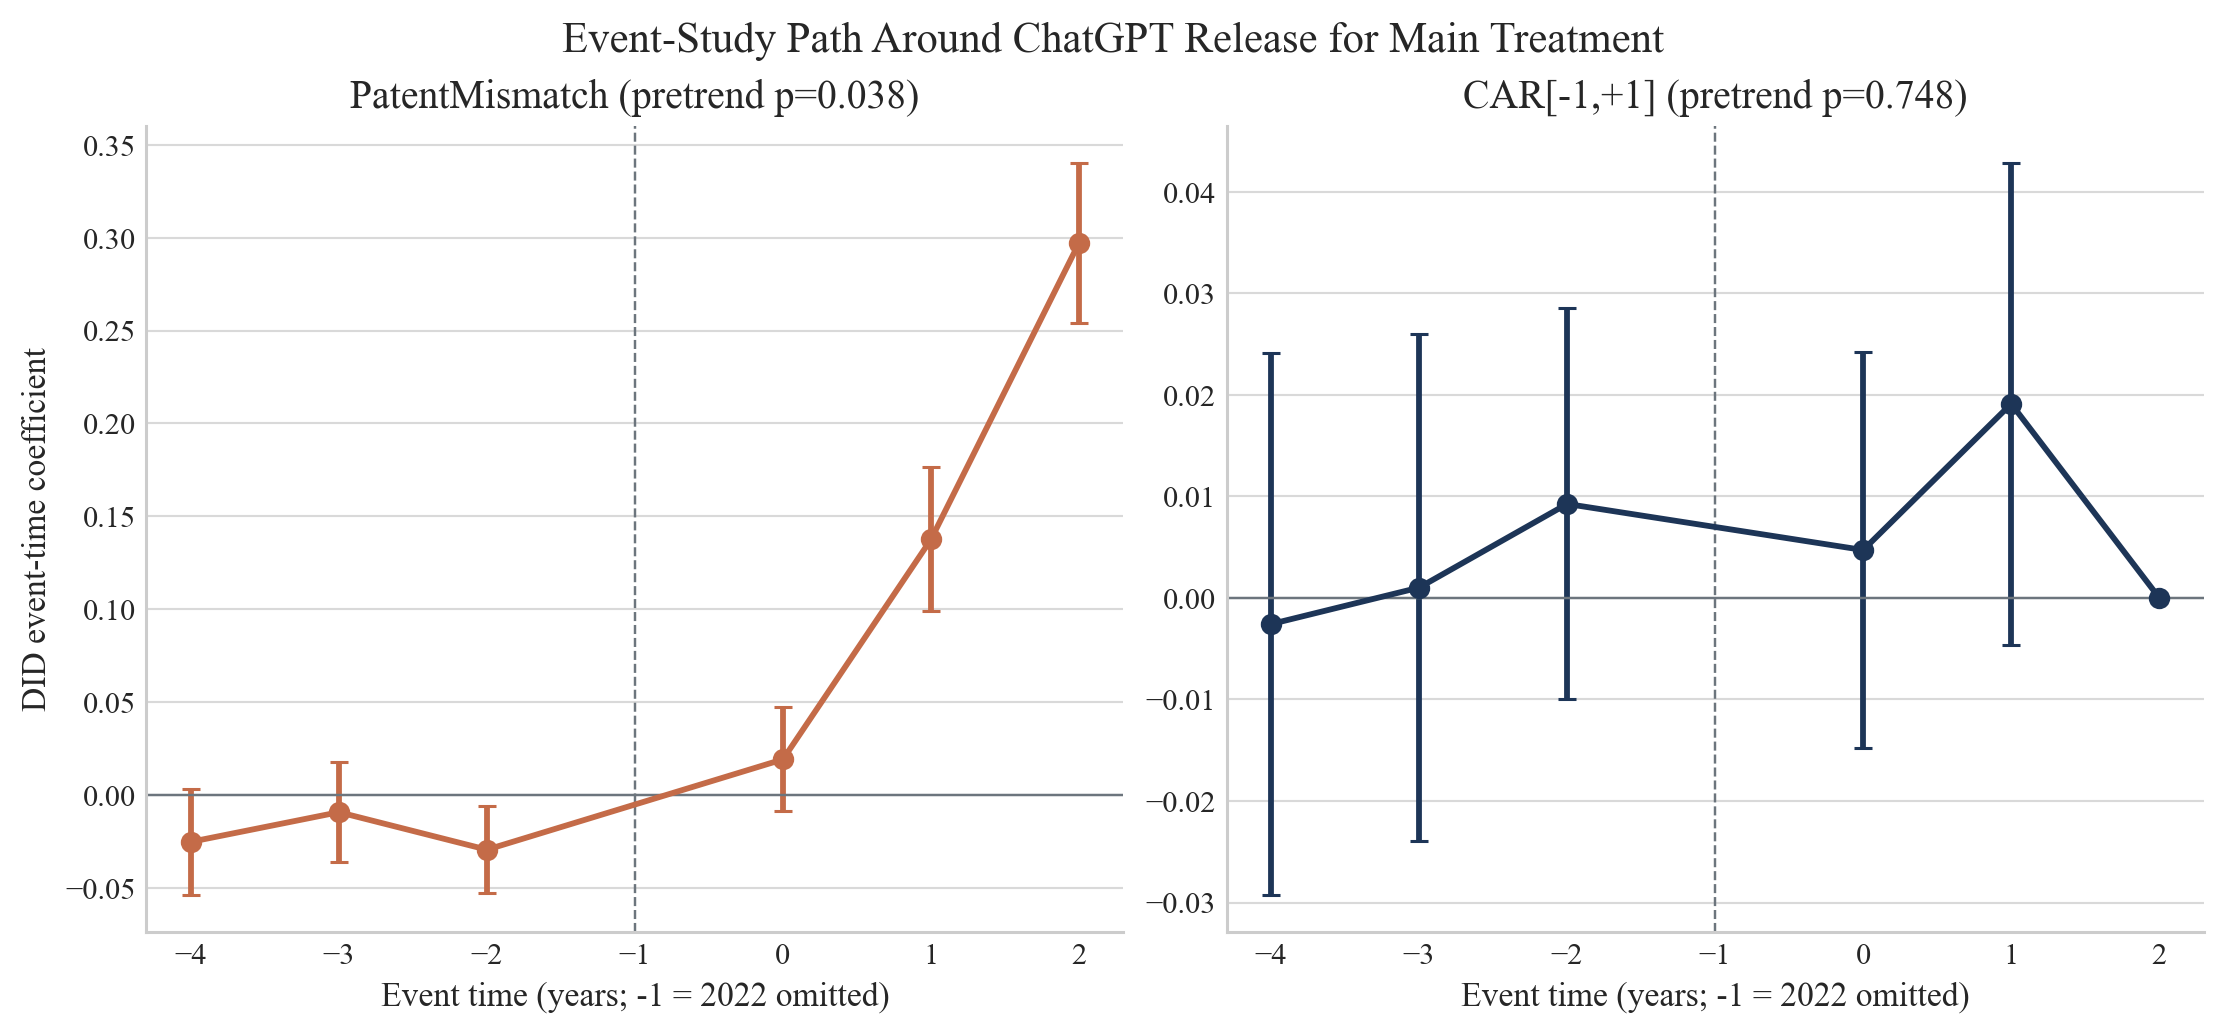
\includegraphics[width=\textwidth]{figures/figureC1.png}
\caption{Event-study path around the release of ChatGPT}
\label{fig:appendix_chatgpt_eventstudy}
\caption*{\footnotesize This figure plots the event-time coefficients for the baseline post-ChatGPT treatment around late 2022. The left panel reports PatentMismatch and the right panel reports filing-date CAR[$-1,+1$]. The figure is included as supporting evidence because the PatentMismatch response is visually strong after the break, but the pretrend diagnostics are not clean enough for this design to carry the paper's central identification burden.}
\end{figure}